\documentclass[aspectratio=169]{../latex_main/tntbeamer}  % you can pass all options of the beamer class, e.g., 'handout' or 'aspectratio=43'
\usepackage{dsfont}
\usepackage{bm}
\usepackage[english]{babel}
\usepackage[T1]{fontenc}
%\usepackage[utf8]{inputenc}
\usepackage{graphicx}
\graphicspath{ {./figures/} }
\usepackage{algorithm}
\usepackage[ruled,vlined,algo2e,linesnumbered]{algorithm2e}
\usepackage{hyperref}
\usepackage{booktabs}
\usepackage{mathtools}

\usepackage{amsmath,amssymb}

\DeclareMathOperator*{\argmax}{arg\,max}
\DeclareMathOperator*{\argmin}{arg\,min}

\usepackage{amsbsy}
\newcommand{\vect}[1]{\bm{#1}}
%\newcommand{\vect}[1]{\boldsymbol{#1}}

\usepackage{pgfplots}
\pgfplotsset{compat=1.16}
\usepackage{tikz}
\usetikzlibrary{trees} 
\usetikzlibrary{shapes.geometric}
\usetikzlibrary{positioning,shapes,shadows,arrows,calc,mindmap}
\usetikzlibrary{positioning,fadings,through}
\usetikzlibrary{decorations.pathreplacing}
\usetikzlibrary{intersections}
\pgfdeclarelayer{background}
\pgfdeclarelayer{foreground}
\pgfsetlayers{background,main,foreground}
\tikzstyle{activity}=[rectangle, draw=black, rounded corners, text centered, text width=8em]
\tikzstyle{data}=[rectangle, draw=black, text centered, text width=8em]
\tikzstyle{myarrow}=[->, thick, draw=black]

% Define the layers to draw the diagram
\pgfdeclarelayer{background}
\pgfdeclarelayer{foreground}
\pgfsetlayers{background,main,foreground}

% Requires XeLaTeX or LuaLaTeX
%\usepackage{unicode-math}

\usepackage{fontspec}
%\setsansfont{Arial}
\setsansfont{RotisSansSerifStd}[ 
Path=../latex_main/fonts/,
Extension = .otf,
UprightFont = *-Regular,  % or *-Light
BoldFont = *-ExtraBold,  % or *-Bold
ItalicFont = *-Italic
]
\setmonofont{Cascadia Mono}[
Scale=0.8
]

% scale factor adapted; mathrm font added (Benjamin Spitschan @TNT, 2021-06-01)
%\setmathfont[Scale=1.05]{Libertinus Math}
%\setmathrm[Scale=1.05]{Libertinus Math}

% other available math fonts are (not exhaustive)
% Latin Modern Math
% XITS Math
% Libertinus Math
% Asana Math
% Fira Math
% TeX Gyre Pagella Math
% TeX Gyre Bonum Math
% TeX Gyre Schola Math
% TeX Gyre Termes Math

% Literature References
\newcommand{\lit}[2]{\href{#2}{\footnotesize\color{black!60}[#1]}}

%%% Beamer Customization
%----------------------------------------------------------------------
% (Don't) Show sections in frame header. Options: 'sections', 'sections light', empty
\setbeamertemplate{headline}{empty}

% Add header logo for normal frames
\setheaderimage{
	% 
\includegraphics[height=\logoheight]{figures/TNT_darkv4.pdf}
	
\includegraphics[height=\logoheight]{../latex_main/figures/luh_logo_rgb_0_80_155.pdf}
	% 
\includegraphics[height=\logoheight]{figures/logo_tntluh.pdf}
}

% Header logo for title page
\settitleheaderimage{
	% 
\includegraphics[height=\logoheight]{figures/TNT_darkv4.pdf}
	
\includegraphics[height=\logoheight]{../latex_main/figures/luh_logo_rgb_0_80_155.pdf}
	% 
\includegraphics[height=\logoheight]{figures/logo_tntluh.pdf}
}

% Title page: tntdefault 
\setbeamertemplate{title page}[tntdefault]  % or luhstyle
% Add optional title image here
%\addtitlepageimagedefault{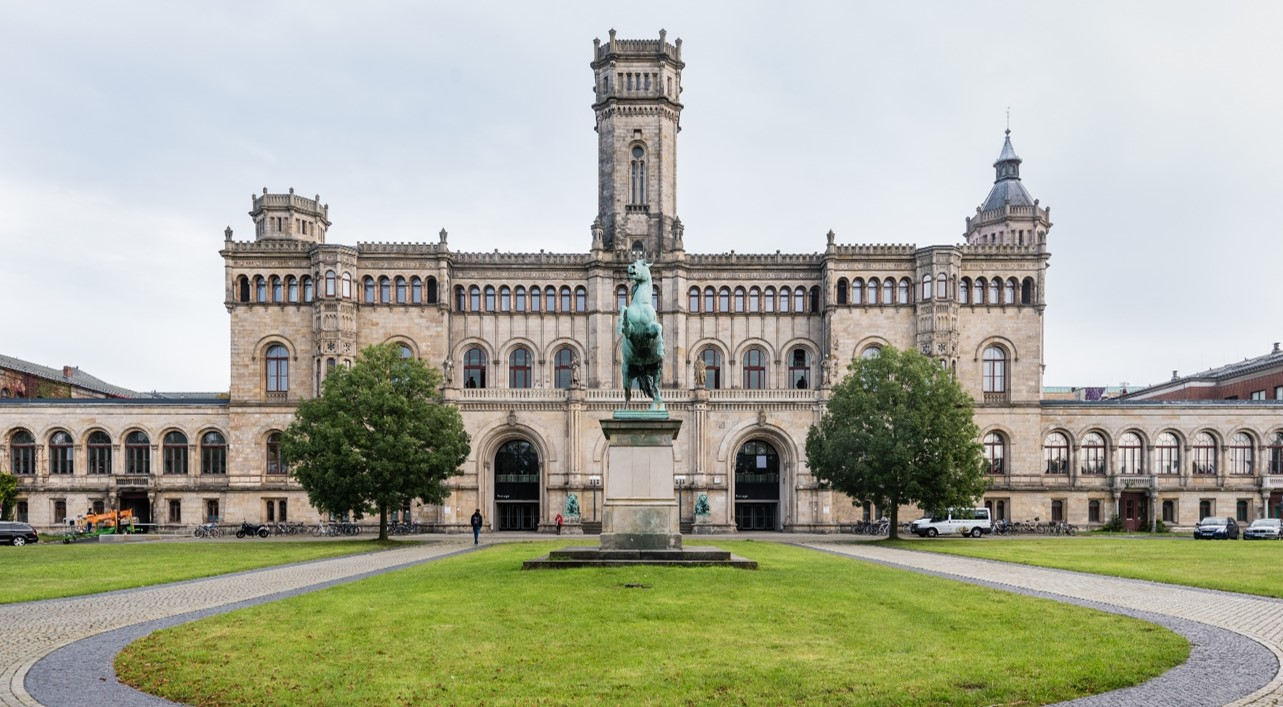
\includegraphics[width=0.65\textwidth]{figures/luh_default_presentation_title_image.jpg}}

% Title page: luhstyle
% \setbeamertemplate{title page}[luhstyle]
% % Add optional title image here
% \addtitlepageimage{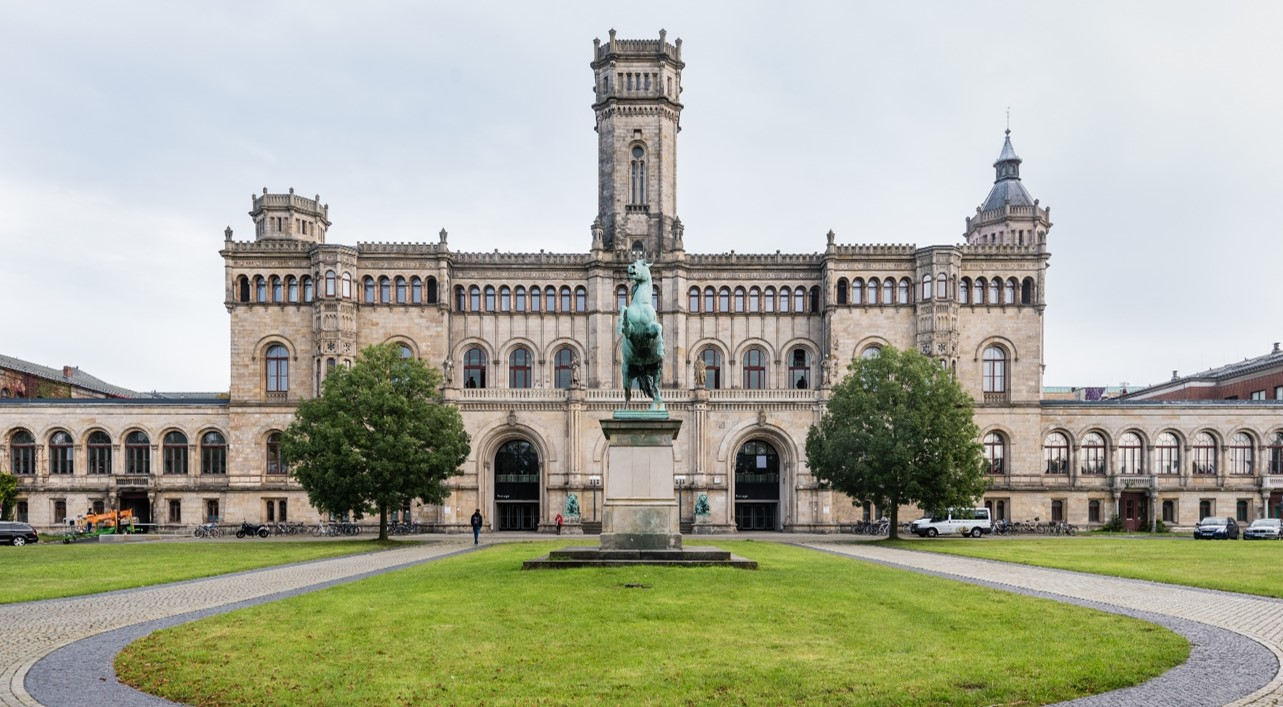
\includegraphics[width=0.75\textwidth]{figures/luh_default_presentation_title_image.jpg}}

\author[Abedjan \& Lindauer]{Ziawasch Abedjan \& Marius Lindauer\\[1em]
	
\includegraphics[height=\logoheight]{../latex_main/figures/luh_logo_rgb_0_80_155.pdf}\qquad
	
\includegraphics[height=\logoheight]{../latex_main/figures/DBIS_Kurzlogo.png}\qquad

\includegraphics[height=\logoheight]{../latex_main/figures/TNT_darkv4}\qquad

\includegraphics[height=\logoheight]{../latex_main/figures/L3S.jpg}	}
\date{Summer Term 2022; \hspace{0.5em} {
\includegraphics[height=1.5em]{../latex_main/figures/Cc-by-nc-sa_icon.svg.png}}; based on \href{https://ds100.org/fa21/}{[DS100]}
}


%%% Custom Packages
%----------------------------------------------------------------------
% Create dummy content
\usepackage{blindtext}

% Adds a frame with the current page layout. Just call \layout inside of a frame.
\usepackage{layout}


%%% Macros
%\renewcommand{\vec}[1]{\mathbf{#1}}
% \usepackage{bm}
%\let\vecb\bm

\title[DL:Multi-Layer Perceptron]{DS: Deep Learning}
\subtitle{Multi-Layer Perceptron}

\date{\hspace{0.5em} {
\includegraphics[height=1.5em]{../latex_main/figures/Cc-by-nc-sa_icon.svg.png}}}

\graphicspath{ {./figure/} }
%\institute{}


\begin{document}
	
	\maketitle
	\begin{frame}{Neuron}

        \begin{itemize}
            \item Basic unit of computation in neural networks.
            \item ``Mimics'' the function of neurons in the biological brain.
            \begin{itemize}
                \item Although many people claim that DL is inspired by the biological brains, this link is very weak.
            \end{itemize}
            \item Consists of inputs, weights, (a bias), and an activation function.
        \end{itemize}
       
        \centering
        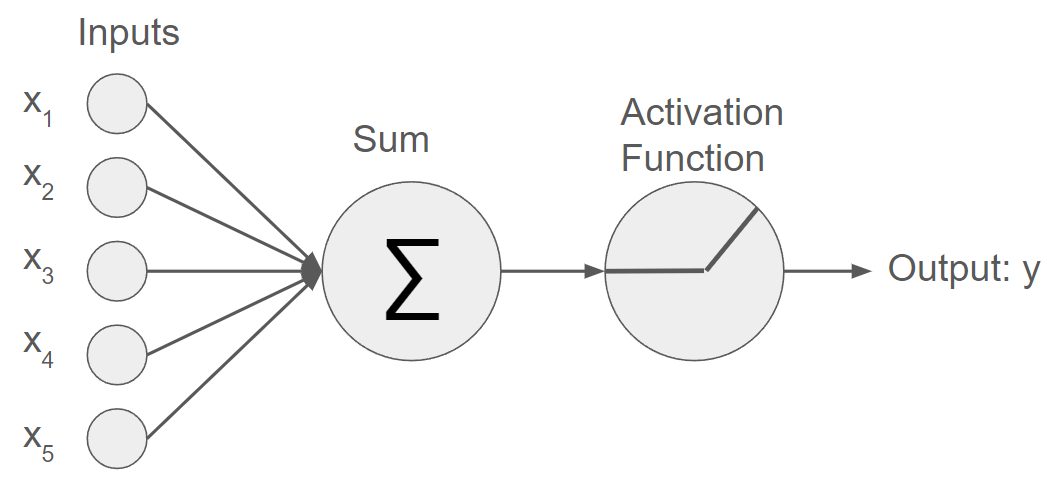
\includegraphics[width=0.6\textwidth]{figures/neuron.png}
                
	\end{frame}

	\begin{frame}{Activation Functions}

        \begin{columns}
            \begin{column}{0.33\textwidth}
                \textbf{Sigmoid}
                \[
                \sigma(x) = \frac{1}{1 + e^{-x}}
                \]
                \begin{itemize}
                    \item Outputs between 0 and 1.
                    \item Useful for probabilities.
                \end{itemize}
            \end{column}

         \begin{column}{0.33\textwidth}
                \textbf{Tanh}
                \[
                \tanh(x) = \frac{e^{x} - e^{-x}}{e^{x} + e^{-x}}
                \]
                \begin{itemize}
                    \item Outputs between -1 and 1.
                    \item Scaled version of the sigmoid.
                \end{itemize}
            \end{column}
            
            \begin{column}{0.33\textwidth}
                \textbf{ReLU}
                \[
                R(x) = \max(0, x)
                \]
                \begin{itemize}
                    \item Non-linear.
                    \item Allows for faster and effective training.
                    \item Most common
                \end{itemize}
            \end{column}
           
        \end{columns}

        More modern activation functions include: Swish, GeLU, Leaky ReLU
                
	\end{frame}

  	\begin{frame}{MLP: Multi-Class Classification}

        \begin{itemize}
            \item Instead of a single neuron, let's combine several of them in a hierarchical level design
            \item The most basic version of a deep neural network (DNN)
            \item Input size depends on your input size
            \item Output depends on your task; here: a single value (e.g., regression)
        \end{itemize}

        \centering
        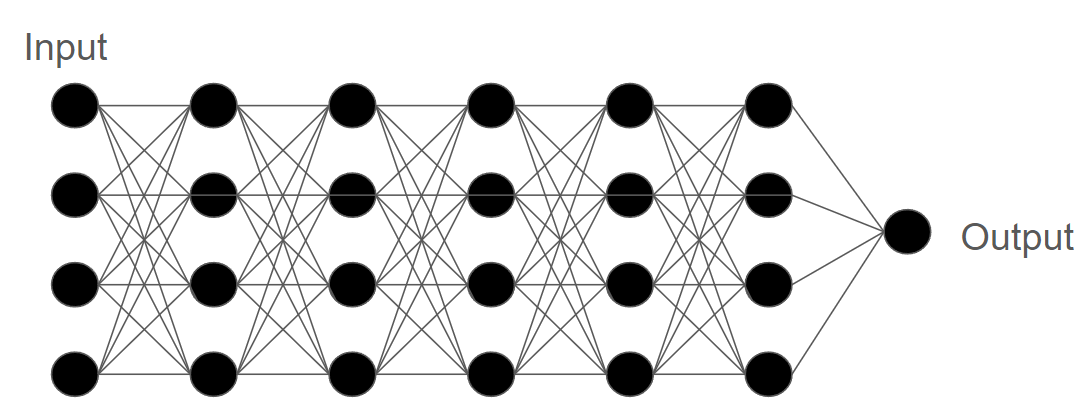
\includegraphics[width=0.6\textwidth]{figures/mlp1.png}
                
	\end{frame}


        \begin{frame}{Layer-wise Representation Learning}

            \centering
            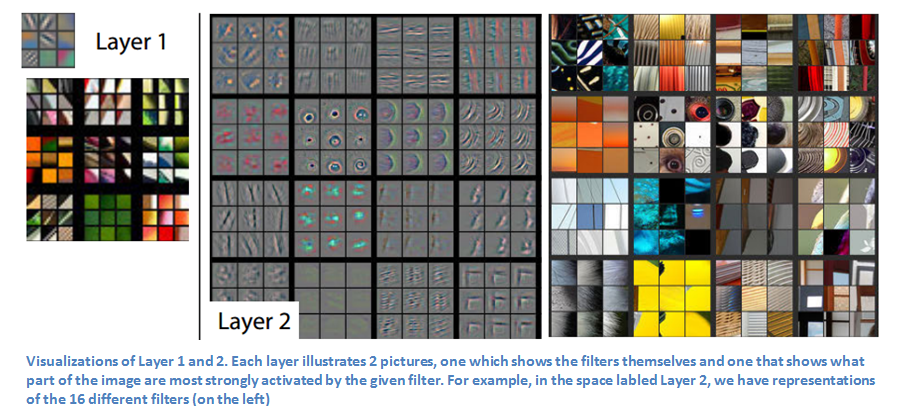
\includegraphics[width=.8\linewidth]{075_deep_learning/figures/deconvnet.png}\\
            Source \href{https://adeshpande3.github.io/The-9-Deep-Learning-Papers-You-Need-To-Know-About.html}{Adit Deshpande}
            
        \end{frame}
        
        \begin{frame}{Layer-wise Representation Learning}

            \centering
            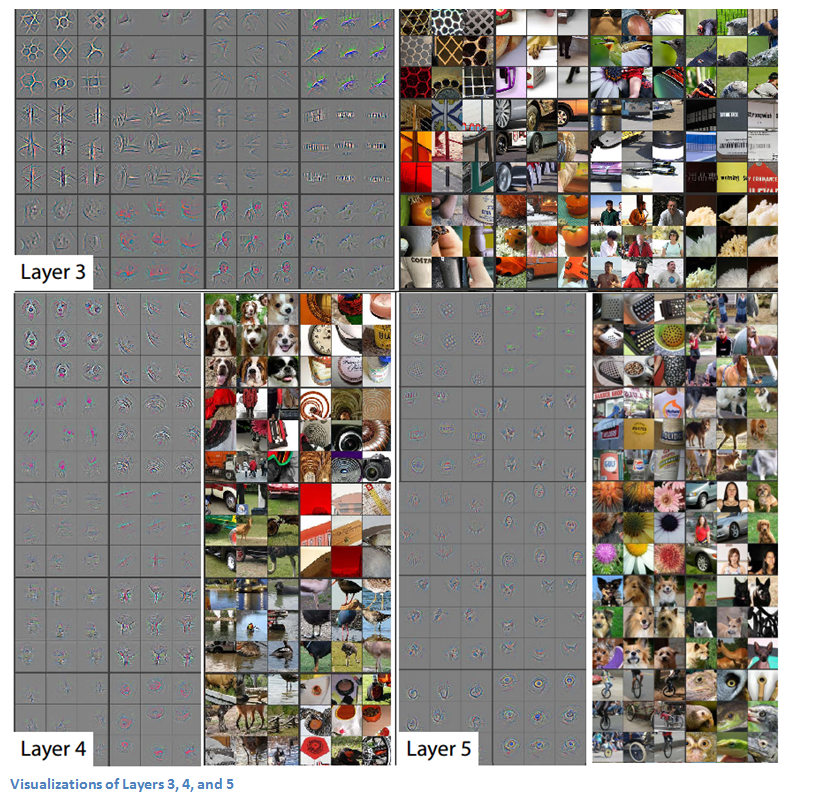
\includegraphics[width=0.42\linewidth]{075_deep_learning/figures/deconvnet2.png}\\
            Source \href{https://adeshpande3.github.io/The-9-Deep-Learning-Papers-You-Need-To-Know-About.html}{Adit Deshpande}
            
        \end{frame}

 	\begin{frame}{Multi-Layer Perceptron: Formally}

        Recursive definition of MLPs:

            \[
            \textbf{y}^{(l)} = \sigma({\Theta}^{(l)} \textbf{y}^{(l-1)} + \textbf{b}^{(l)})
            \]
            
            where:
            \begin{itemize}
                \item \( \textbf{y}^{(l)} \) is the output vector from layer \( l \)
                \item \( {\Theta}^{(l)} \) represents the weight matrix for layer \( l \)
                \item \( \textbf{y}^{(l-1)} \) is the output vector from the previous layer \( l-1 \)
                \item \( \textbf{b}^{(l)} \) is the bias vector for layer \( l \)
                \item \( \sigma \) is the activation function (e.g., ReLU)
            \end{itemize}
	\end{frame}


  	\begin{frame}{Multi-Layer Perceptron: Classification via Softmax}

        \begin{itemize}
            \item 1 output neuron for each output
            \item[$\leadsto$] Softmax to transform into pseudo-probabilities
        \end{itemize}

        \[
        \text{Softmax}(z_i) = \frac{e^{z_i}}{\sum_{j=1}^{K} e^{z_j}}
        \]
        
        where \( z_i \) represents the input to the softmax function for class \( i \), and \( K \) is the total number of classes.

        \centering
        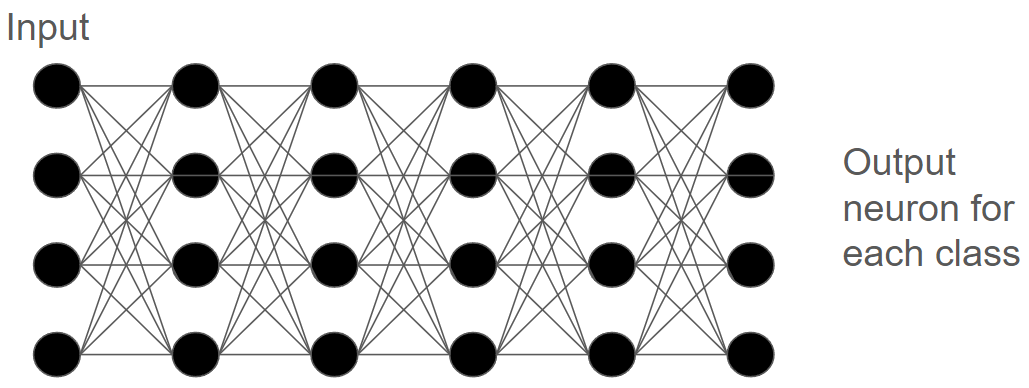
\includegraphics[width=0.5\textwidth]{figures/mlp2.png}
                
	\end{frame}

  	\begin{frame}{Classification Loss: Cross-Entropy}

        \begin{itemize}
            \item Typical loss for DNNs on classification tasks
            \item Easy to learn on 
            \begin{itemize}
                \item better than accuracy because we can follow the gradient of it 
            \end{itemize}
            \item Important: Check that your validation loss (e.g., accuracy) also improves while training your DNN
        \end{itemize}

        \[
        \text{Cross-Entropy Loss} = -\sum_{i=1}^{C} y_i \log(p_i)
        \]
        
        where \( y_i \) is the true label (1 or 0, indicating whether the class label \( i \) is the correct classification), and \( p_i \) is the predicted probability of the observation being of class \( i \).
                
	\end{frame}

 	
\end{document}